\section{Definition and Framework}
\label{sec:definition&framework}

\subsection{Problem Definition}
\label{sec:definition}

An instance consists of some property-value descriptions about a real-world object. A pair of distinct instances $a$ and $b$ match if they refer to the same object, denoted by $(a,b)\in\mathcal{R}$. In LOD, \texttt{owl:sameAs} links are established between matching instances. When establishing such links, we usually consider a pair of data sources each time.
\begin{definition}[Instance Matching]
Given two data sources $A$ and $B$ as input, the goal of instance matching is to compute the set $\mathcal{M}=\{(a,b)|(a,b)\in A \times B, (a,b)\in\mathcal{R}\}$.
\end{definition}
According to the definition of instance matching, the problem of finding matching instance pairs can be formalized as a binary classification problem.
\begin{definition}[Instance Matching as Binary Classification]
Given two data sources $A$ and $B$, the goal of instance matching is to find a classifier $\mathcal{C}:(a, b) \to\{-1, 1\}$ for $(a, b)\in A \times B$ such that $\mathcal{C}$ maps the non-matching instance pairs to class $-1$ and the matching ones to the class $1$.
\end{definition}
The binary classification problem can be solved by traditional machine learning algorithms, which require multidimensional features as the input. In the problem of instance matching, we extract a feature vector from each instance pair $(a, b)$.
\begin{definition}[Similarity Vector of Instance Pairs]
The n-dimensional feature vector $v$ of an instance pair $(a, b)$ consists of $n$ various similarities of instance $a$ and $b$. Dimension $v_i =d_i (a, b)$, where $d_i$ is the $i$th similarity metric function for $(a, b)$.
\end{definition}
The feature vector of an instance pair indicates the similarities of the two instances, which are computed by several metric functions. Some existing instance matching (record linkage\cite{elmagarmid2007duplicate}) approaches also extract such a feature vector for classification, while each $d_i$ computes the similarity of two values, one from each instance, that belong to a pair of matching properties (fields). Unlike these approaches, our similarity metric functions are based on the property-independent literal information extracted from each instance. The literal information $l=\{l_1 , l_2 , \dots , l_n\}$ is similar to a virtual document generated from an instance. For an instance pair $(a, b)$, a similarity metric function $d_i$ maps the extracted literal information pair $(l^a_i, l^b_i)$ to a real number in the range of $[0, 1]$.

\subsection{Framework}
\label{sec:framework}

\begin{figure}[t]
  \centering
  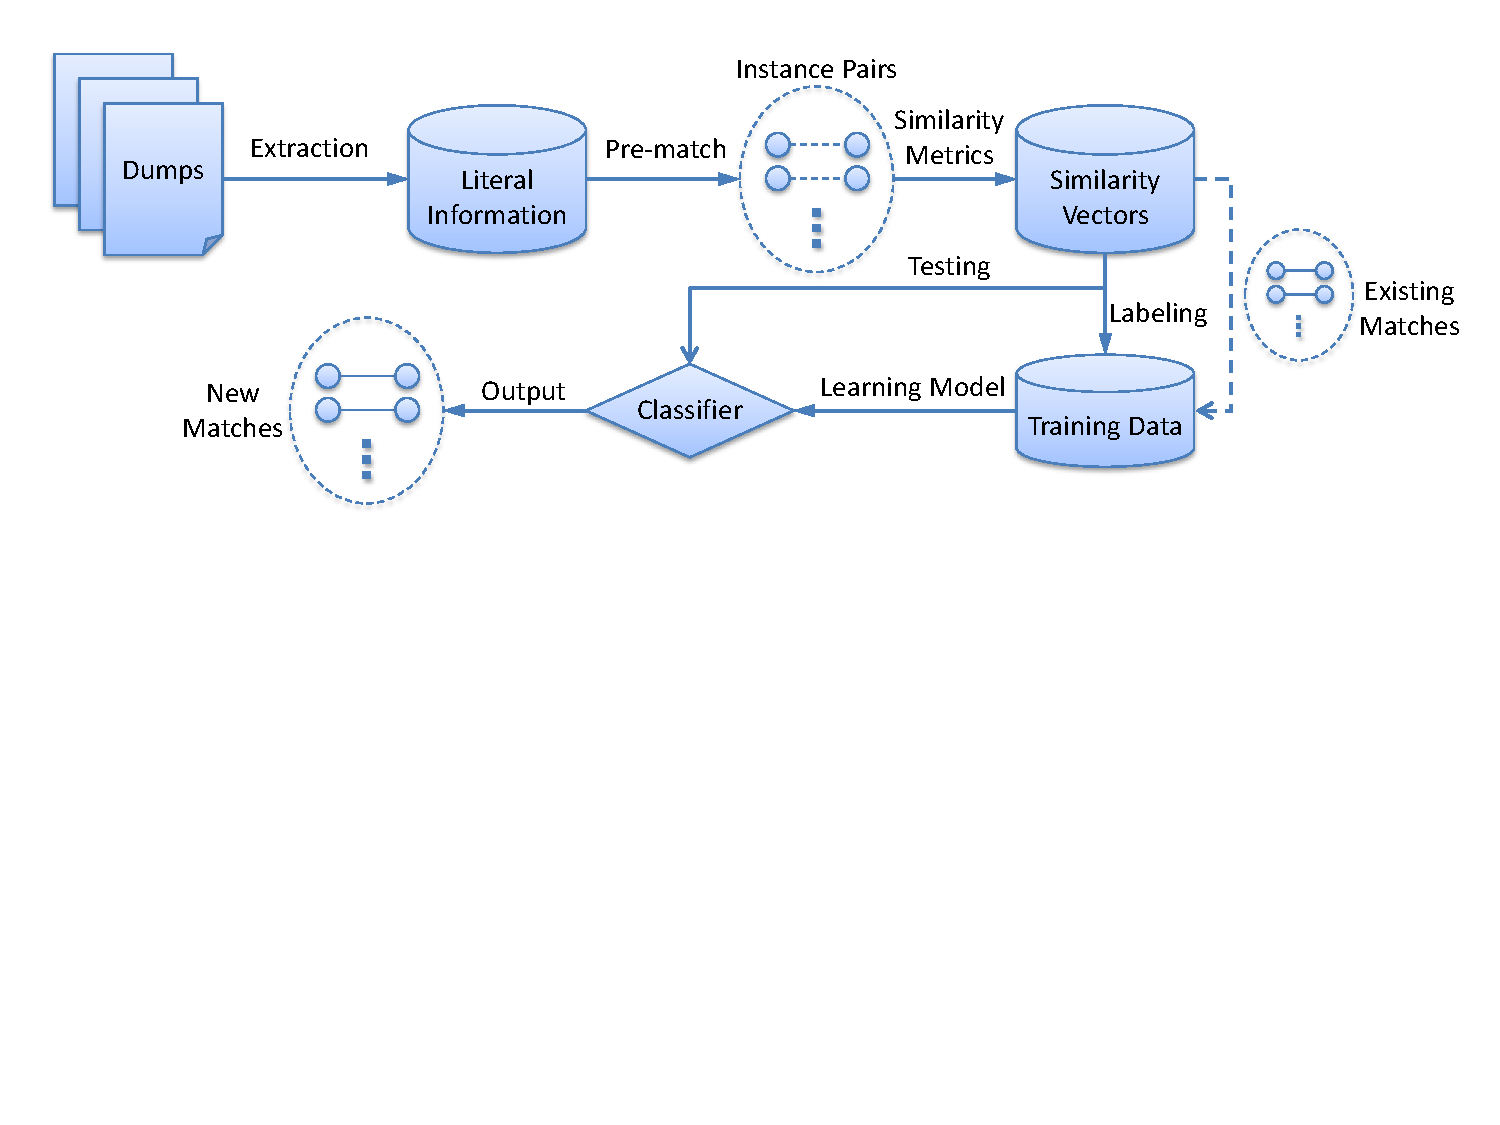
\includegraphics[width=1\textwidth]{figures/framework}
  \caption{Overview of the framework}
  \label{fig:framework}
\end{figure}
The framework of our approach is shown in Figure \ref{fig:framework}. We extract literal information for each instance from the property-value descriptions. To get sufficient literal information for the similarity metrics, we conduct the following preprocessing for each property-value pair:
\begin{itemize}
\item A real-world object may be represented by an instance or a piece of text. For consistency, if the value is a URI which represents another instance, we will replace it by the label of that instance. Most of the instances have a label value which usually belongs to the property \texttt{rdfs:label} or some other common properties\cite{ell2011labels}. If the label of an instance is unavailable, we can replace it by its text description.
\item We will also replace each property by its label. If the label is unavailable, we will use the last token (normalized) of the URI instead, e.g., \textquotedblleft place of death \textquotedblright for \texttt{fb:place\_of\_death}.
\end{itemize}
For data sources $A$ and $B$ which contain $|A|$ and $|B|$ instances respectively, there are $|A|\times|B|$ possible instance pairs. This is unacceptable since both $|A|$ and $|B|$ can be one million or even larger. We use a simple pre-match method to sift the possible matching pairs. An inverted index is built for instances of some key words in their descriptions. The instances sharing the same keys in the index are considered to be candidate matching instances. Our preliminary experiments show that this sifting method can greatly reduce the number of pairs  to test for a match, without losing much recall (the recall is over $0.9$).

After preprocessing and literal information extraction, we compute the similarity vectors for the candidates. To train a binary classifier based on the similarity vectors, we need to label some of them into class -1 (non-matching) or class 1 (matching). Thus the problem of instance matching can be solved by classifying the unlabeled instance pairs. The existing matching instance pairs in LOD can be considered as labeled data which may help to train the classifier. We employ a transfer learning algorithm to improve the effect of the helping.
